
%% bare_jrnl.tex
%% V1.4a
%% 2014/09/17
%% by Michael Shell
%% see http://www.michaelshell.org/
%% for current contact information.
%%
%% This is a skeleton file demonstrating the use of IEEEtran.cls
%% (requires IEEEtran.cls version 1.8a or later) with an IEEE
%% journal paper.
%%
%% Support sites:
%% http://www.michaelshell.org/tex/ieeetran/
%% http://www.ctan.org/tex-archive/macros/latex/contrib/IEEEtran/
%% and
%% http://www.ieee.org/

%%*************************************************************************
%% Legal Notice:
%% This code is offered as-is without any warranty either expressed or
%% implied; without even the implied warranty of MERCHANTABILITY or
%% FITNESS FOR A PARTICULAR PURPOSE! 
%% User assumes all risk.
%% In no event shall IEEE or any contributor to this code be liable for
%% any damages or losses, including, but not limited to, incidental,
%% consequential, or any other damages, resulting from the use or misuse
%% of any information contained here.
%%
%% All comments are the opinions of their respective authors and are not
%% necessarily endorsed by the IEEE.
%%
%% This work is distributed under the LaTeX Project Public License (LPPL)
%% ( http://www.latex-project.org/ ) version 1.3, and may be freely used,
%% distributed and modified. A copy of the LPPL, version 1.3, is included
%% in the base LaTeX documentation of all distributions of LaTeX released
%% 2003/12/01 or later.
%% Retain all contribution notices and credits.
%% ** Modified files should be clearly indicated as such, including  **
%% ** renaming them and changing author support contact information. **
%%
%% File list of work: IEEEtran.cls, IEEEtran_HOWTO.pdf, bare_adv.tex,
%%                    bare_conf.tex, bare_jrnl.tex, bare_conf_compsoc.tex,
%%                    bare_jrnl_compsoc.tex, bare_jrnl_transmag.tex
%%*************************************************************************


% *** Authors should verify (and, if needed, correct) their LaTeX system  ***
% *** with the testflow diagnostic prior to trusting their LaTeX platform ***
% *** with production work. IEEE's font choices and paper sizes can       ***
% *** trigger bugs that do not appear when using other class files.       ***                          ***
% The testflow support page is at:
% http://www.michaelshell.org/tex/testflow/



\documentclass[journal]{IEEEtran}
%
% If IEEEtran.cls has not been installed into the LaTeX system files,
% manually specify the path to it like:
% \documentclass[journal]{../sty/IEEEtran}


% *** CITATION PACKAGES ***
%
\usepackage{cite}
% cite.sty was written by Donald Arseneau
% V1.6 and later of IEEEtran pre-defines the format of the cite.sty package
% \cite{} output to follow that of IEEE. Loading the cite package will
% result in citation numbers being automatically sorted and properly
% "compressed/ranged". e.g., [1], [9], [2], [7], [5], [6] without using
% cite.sty will become [1], [2], [5]--[7], [9] using cite.sty. cite.sty's
% \cite will automatically add leading space, if needed. Use cite.sty's
% noadjust option (cite.sty V3.8 and later) if you want to turn this off
% such as if a citation ever needs to be enclosed in parenthesis.
% cite.sty is already installed on most LaTeX systems. Be sure and use
% version 5.0 (2009-03-20) and later if using hyperref.sty.
% The latest version can be obtained at:
% http://www.ctan.org/tex-archive/macros/latex/contrib/cite/
% The documentation is contained in the cite.sty file itself.


% *** GRAPHICS RELATED PACKAGES ***
%
\ifCLASSINFOpdf
  \usepackage[pdftex]{graphicx}
  % declare the path(s) where your graphic files are
  % \graphicspath{{../pdf/}{../jpeg/}}
  % and their extensions so you won't have to specify these with
  % every instance of \includegraphics
  % \DeclareGraphicsExtensions{.pdf,.jpeg,.png}
\else
  % or other class option (dvipsone, dvipdf, if not using dvips). graphicx
  % will default to the driver specified in the system graphics.cfg if no
  % driver is specified.
  % \usepackage[dvips]{graphicx}
  % declare the path(s) where your graphic files are
  % \graphicspath{{../eps/}}
  % and their extensions so you won't have to specify these with
  % every instance of \includegraphics
  % \DeclareGraphicsExtensions{.eps}
\fi
% graphicx was written by David Carlisle and Sebastian Rahtz. It is
% required if you want graphics, photos, etc. graphicx.sty is already
% installed on most LaTeX systems. The latest version and documentation
% can be obtained at: 
% http://www.ctan.org/tex-archive/macros/latex/required/graphics/
% Another good source of documentation is "Using Imported Graphics in
% LaTeX2e" by Keith Reckdahl which can be found at:
% http://www.ctan.org/tex-archive/info/epslatex/
%
% latex, and pdflatex in dvi mode, support graphics in encapsulated
% postscript (.eps) format. pdflatex in pdf mode supports graphics
% in .pdf, .jpeg, .png and .mps (metapost) formats. Users should ensure
% that all non-photo figures use a vector format (.eps, .pdf, .mps) and
% not a bitmapped formats (.jpeg, .png). IEEE frowns on bitmapped formats
% which can result in "jaggedy"/blurry rendering of lines and letters as
% well as large increases in file sizes.
%
% You can find documentation about the pdfTeX application at:
% http://www.tug.org/applications/pdftex





% *** MATH PACKAGES ***
%
\usepackage[cmex10]{amsmath}
% A popular package from the American Mathematical Society that provides
% many useful and powerful commands for dealing with mathematics. If using
% it, be sure to load this package with the cmex10 option to ensure that
% only type 1 fonts will utilized at all point sizes. Without this option,
% it is possible that some math symbols, particularly those within
% footnotes, will be rendered in bitmap form which will result in a
% document that can not be IEEE Xplore compliant!
%
% Also, note that the amsmath package sets \interdisplaylinepenalty to 10000
% thus preventing page breaks from occurring within multiline equations. Use:
%\interdisplaylinepenalty=2500
% after loading amsmath to restore such page breaks as IEEEtran.cls normally
% does. amsmath.sty is already installed on most LaTeX systems. The latest
% version and documentation can be obtained at:
% http://www.ctan.org/tex-archive/macros/latex/required/amslatex/math/





% *** SPECIALIZED LIST PACKAGES ***
%
%\usepackage{algorithmic}
% algorithmic.sty was written by Peter Williams and Rogerio Brito.
% This package provides an algorithmic environment fo describing algorithms.
% You can use the algorithmic environment in-text or within a figure
% environment to provide for a floating algorithm. Do NOT use the algorithm
% floating environment provided by algorithm.sty (by the same authors) or
% algorithm2e.sty (by Christophe Fiorio) as IEEE does not use dedicated
% algorithm float types and packages that provide these will not provide
% correct IEEE style captions. The latest version and documentation of
% algorithmic.sty can be obtained at:
% http://www.ctan.org/tex-archive/macros/latex/contrib/algorithms/
% There is also a support site at:
% http://algorithms.berlios.de/index.html
% Also of interest may be the (relatively newer and more customizable)
% algorithmicx.sty package by Szasz Janos:
% http://www.ctan.org/tex-archive/macros/latex/contrib/algorithmicx/




% *** ALIGNMENT PACKAGES ***
%
%\usepackage{array}
% Frank Mittelbach's and David Carlisle's array.sty patches and improves
% the standard LaTeX2e array and tabular environments to provide better
% appearance and additional user controls. As the default LaTeX2e table
% generation code is lacking to the point of almost being broken with
% respect to the quality of the end results, all users are strongly
% advised to use an enhanced (at the very least that provided by array.sty)
% set of table tools. array.sty is already installed on most systems. The
% latest version and documentation can be obtained at:
% http://www.ctan.org/tex-archive/macros/latex/required/tools/


% IEEEtran contains the IEEEeqnarray family of commands that can be used to
% generate multiline equations as well as matrices, tables, etc., of high
% quality.




% *** SUBFIGURE PACKAGES ***
%\ifCLASSOPTIONcompsoc
%  \usepackage[caption=false,font=normalsize,labelfont=sf,textfont=sf]{subfig}
%\else
%  \usepackage[caption=false,font=footnotesize]{subfig}
%\fi
% subfig.sty, written by Steven Douglas Cochran, is the modern replacement
% for subfigure.sty, the latter of which is no longer maintained and is
% incompatible with some LaTeX packages including fixltx2e. However,
% subfig.sty requires and automatically loads Axel Sommerfeldt's caption.sty
% which will override IEEEtran.cls' handling of captions and this will result
% in non-IEEE style figure/table captions. To prevent this problem, be sure
% and invoke subfig.sty's "caption=false" package option (available since
% subfig.sty version 1.3, 2005/06/28) as this is will preserve IEEEtran.cls
% handling of captions.
% Note that the Computer Society format requires a larger sans serif font
% than the serif footnote size font used in traditional IEEE formatting
% and thus the need to invoke different subfig.sty package options depending
% on whether compsoc mode has been enabled.
%
% The latest version and documentation of subfig.sty can be obtained at:
% http://www.ctan.org/tex-archive/macros/latex/contrib/subfig/




% *** FLOAT PACKAGES ***
%
%\usepackage{fixltx2e}
% fixltx2e, the successor to the earlier fix2col.sty, was written by
% Frank Mittelbach and David Carlisle. This package corrects a few problems
% in the LaTeX2e kernel, the most notable of which is that in current
% LaTeX2e releases, the ordering of single and double column floats is not
% guaranteed to be preserved. Thus, an unpatched LaTeX2e can allow a
% single column figure to be placed prior to an earlier double column
% figure. The latest version and documentation can be found at:
% http://www.ctan.org/tex-archive/macros/latex/base/


%\usepackage{stfloats}
% stfloats.sty was written by Sigitas Tolusis. This package gives LaTeX2e
% the ability to do double column floats at the bottom of the page as well
% as the top. (e.g., "\begin{figure*}[!b]" is not normally possible in
% LaTeX2e). It also provides a command:
%\fnbelowfloat
% to enable the placement of footnotes below bottom floats (the standard
% LaTeX2e kernel puts them above bottom floats). This is an invasive package
% which rewrites many portions of the LaTeX2e float routines. It may not work
% with other packages that modify the LaTeX2e float routines. The latest
% version and documentation can be obtained at:
% http://www.ctan.org/tex-archive/macros/latex/contrib/sttools/
% Do not use the stfloats baselinefloat ability as IEEE does not allow
% \baselineskip to stretch. Authors submitting work to the IEEE should note
% that IEEE rarely uses double column equations and that authors should try
% to avoid such use. Do not be tempted to use the cuted.sty or midfloat.sty
% packages (also by Sigitas Tolusis) as IEEE does not format its papers in
% such ways.
% Do not attempt to use stfloats with fixltx2e as they are incompatible.
% Instead, use Morten Hogholm'a dblfloatfix which combines the features
% of both fixltx2e and stfloats:
%
% \usepackage{dblfloatfix}
% The latest version can be found at:
% http://www.ctan.org/tex-archive/macros/latex/contrib/dblfloatfix/




%\ifCLASSOPTIONcaptionsoff
%  \usepackage[nomarkers]{endfloat}
% \let\MYoriglatexcaption\caption
% \renewcommand{\caption}[2][\relax]{\MYoriglatexcaption[#2]{#2}}
%\fi
% endfloat.sty was written by James Darrell McCauley, Jeff Goldberg and 
% Axel Sommerfeldt. This package may be useful when used in conjunction with 
% IEEEtran.cls'  captionsoff option. Some IEEE journals/societies require that
% submissions have lists of figures/tables at the end of the paper and that
% figures/tables without any captions are placed on a page by themselves at
% the end of the document. If needed, the draftcls IEEEtran class option or
% \CLASSINPUTbaselinestretch interface can be used to increase the line
% spacing as well. Be sure and use the nomarkers option of endfloat to
% prevent endfloat from "marking" where the figures would have been placed
% in the text. The two hack lines of code above are a slight modification of
% that suggested by in the endfloat docs (section 8.4.1) to ensure that
% the full captions always appear in the list of figures/tables - even if
% the user used the short optional argument of \caption[]{}.
% IEEE papers do not typically make use of \caption[]'s optional argument,
% so this should not be an issue. A similar trick can be used to disable
% captions of packages such as subfig.sty that lack options to turn off
% the subcaptions:
% For subfig.sty:
% \let\MYorigsubfloat\subfloat
% \renewcommand{\subfloat}[2][\relax]{\MYorigsubfloat[]{#2}}
% However, the above trick will not work if both optional arguments of
% the \subfloat command are used. Furthermore, there needs to be a
% description of each subfigure *somewhere* and endfloat does not add
% subfigure captions to its list of figures. Thus, the best approach is to
% avoid the use of subfigure captions (many IEEE journals avoid them anyway)
% and instead reference/explain all the subfigures within the main caption.
% The latest version of endfloat.sty and its documentation can obtained at:
% http://www.ctan.org/tex-archive/macros/latex/contrib/endfloat/
%
% The IEEEtran \ifCLASSOPTIONcaptionsoff conditional can also be used
% later in the document, say, to conditionally put the References on a 
% page by themselves.




% *** PDF, URL AND HYPERLINK PACKAGES ***
%
%\usepackage{url}
% url.sty was written by Donald Arseneau. It provides better support for
% handling and breaking URLs. url.sty is already installed on most LaTeX
% systems. The latest version and documentation can be obtained at:
% http://www.ctan.org/tex-archive/macros/latex/contrib/url/
% Basically, \url{my_url_here}.




% *** Do not adjust lengths that control margins, column widths, etc. ***
% *** Do not use packages that alter fonts (such as pslatex).         ***
% There should be no need to do such things with IEEEtran.cls V1.6 and later.
% (Unless specifically asked to do so by the journal or conference you plan
% to submit to, of course. )


% correct bad hyphenation here
\hyphenation{op-tical net-works semi-conduc-tor}


\begin{document}
%
% paper title
% Titles are generally capitalized except for words such as a, an, and, as,
% at, but, by, for, in, nor, of, on, or, the, to and up, which are usually
% not capitalized unless they are the first or last word of the title.
% Linebreaks \\ can be used within to get better formatting as desired.
% Do not put math or special symbols in the title.
\title{Syllable Recognition and Lattice Transduction for Low-resource Keyword Search}
%
%
% author names and IEEE memberships
% note positions of commas and nonbreaking spaces ( ~ ) LaTeX will not break
% a structure at a ~ so this keeps an author's name from being broken across
% two lines.
% use \thanks{} to gain access to the first footnote area
% a separate \thanks must be used for each paragraph as LaTeX2e's \thanks
% was not built to handle multiple paragraphs
%

\author{Hang~Su,~\IEEEmembership{Student Member,~IEEE,}
        James Hieronymus,~\IEEEmembership{Member,~IEEE}% <-this % stops a space
\thanks{H. Su is with the Department of Electrical Engineering and Computer Science,
University of California, Berkeley, CA 94704, USA. e-mail: suhang3240@gmail.com}% <-this % stops a space
\thanks{J. Hieronymus is with International Computer Science Institute.}}

% note the % following the last \IEEEmembership and also \thanks - 
% these prevent an unwanted space from occurring between the last author name
% and the end of the author line. i.e., if you had this:
% 
% \author{....lastname \thanks{...} \thanks{...} }
%                     ^------------^------------^----Do not want these spaces!
%
% a space would be appended to the last name and could cause every name on that
% line to be shifted left slightly. This is one of those "LaTeX things". For
% instance, "\textbf{A} \textbf{B}" will typeset as "A B" not "AB". To get
% "AB" then you have to do: "\textbf{A}\textbf{B}"
% \thanks is no different in this regard, so shield the last } of each \thanks
% that ends a line with a % and do not let a space in before the next \thanks.
% Spaces after \IEEEmembership other than the last one are OK (and needed) as
% you are supposed to have spaces between the names. For what it is worth,
% this is a minor point as most people would not even notice if the said evil
% space somehow managed to creep in.



% The paper headers
\markboth{IEEE/ACM TRANSACTIONS ON AUDIO, SPEECH, AND LANGUAGE PROCESSING, VOL. XX, NO. XX, MONTH YEAR}{}
% The only time the second header will appear is for the odd numbered pages
% after the title page when using the twoside option.
% 
% *** Note that you probably will NOT want to include the author's ***
% *** name in the headers of peer review papers.                   ***
% You can use \ifCLASSOPTIONpeerreview for conditional compilation here if
% you desire.

% If you want to put a publisher's ID mark on the page you can do it like
% this:
%\IEEEpubid{0000--0000/00\$00.00~\copyright~2014 IEEE}
% Remember, if you use this you must call \IEEEpubidadjcol in the second
% column for its text to clear the IEEEpubid mark.

% make the title area
\maketitle

% As a general rule, do not put math, special symbols or citations
% in the abstract or keywords.
\begin{abstract}
Low-resource speech recognition and keyword search (KWS) are important topics for speech technologies. However,
their performance often suffer from out-of-vocabulary (OOV) keywords. Subword units like syllables are useful 
in handling this issue. This report introduces a weighted finite state transducer (WFST) based syllable transduction 
framework for OOV handling in KWS. Experiments on languages provided by the Babel project\footnote{Supported by 
the Intelligence Advanced Research Projects Activity (IARPA) via 
Department of Defense US Army Research Laboratory contract number W911NF-12-C-0014. The U.S. Government is 
authorized to reproduce and distribute reprints for Governmental purposes notwithstanding any
copyright annotation thereon. Disclaimer: The views and conclusions contained herein are those of the 
authors and should not be interpreted as necessarily representing the official policies or endorsements, 
either expressed or implied, of IARPA, DoD/ARL, or the U.S. Government.} are presented, and it is shown that 
syllable transduction can effectively spot OOV keywords. Combination of this approach with two
other OOV handling methods further improves keyword search performance.
\end{abstract}

% Note that keywords are not normally used for peerreview papers.
\begin{IEEEkeywords}
Syllable, Lattice Transduction, Low-resource, Keyword Search
\end{IEEEkeywords}


% For peer review papers, you can put extra information on the cover
% page as needed:
% \ifCLASSOPTIONpeerreview
% \begin{center} \bfseries EDICS Category: 3-BBND \end{center}
% \fi
%
% For peerreview papers, this IEEEtran command inserts a page break and
% creates the second title. It will be ignored for other modes.
\IEEEpeerreviewmaketitle

\section{Introduction}
\IEEEPARstart{N}{owadays}, keyword search in speech/audio is becoming more and more important as lots of multimedia are 
available on the Internet. However, unlike text search, audio/speech search is a much harder task. Researchers 
have been developing KWS systems based on speech recognition technology, which itself is an unsolved 
artificial intelligence problem. Thanks to the progress made by the speech community, speech search is 
becoming a more practical technique in recent years.

Multilingual speech search presents a unique set of challenges, including novel speech sounds, agglomerative 
morphology which causes large vocabularies, and lack of transcribed data for model training. 
Especially, when training data is limited, there will be lots of out-of-vocabulary (OOV) words in the test 
set that makes it impractical to search them without special treatment.

The IARPA Babel program\cite{babel} instantiates this scenario well in providing a limited amount of 
transcribed training data and lexicons for words and syllables in several minority languages. For the 
languages provided so far the numbers of OOV keywords are from 10\% to 25\%. This report investigates 
KWS in low-resources condition, with an emphasis on OOV issue.

The organization of the report is as follows. Section 2 introduces the background of speech recognition and
keyword search, together with two OOV handling methods. Section 3 illustrates the WFST framework for syllable
transduction. Section 4 introduces the BABEL project and Section 5 presents experimental results on several 
languages. Section 6 concludes this work.

\section{Background}
KWS in audio is usually based on speech recognition. A set of audio files and their corresponding 
transcriptions are given as training data to bring up a speech recognizer. Test audio files are then 
transcribed via Automatic Speech Recognition (ASR) and word lattices containing possible transcriptions 
are generated (this procedure is called decoding). Keyword search is conducted based on the produced word lattices.

\subsection{WFST Framework for ASR}
Speech recognition task could be well formulated as a composition task in the framework of weighted finite state 
transducer (WFST). A typical WFST decoding graph generation in speech recognition\cite{mohri2008speech} is 
represented as
\begin{equation}
H \circ C \circ L \circ G
\end{equation}
where $H$, $C$, $L$ and $G$ are WFSTs for a state network of triphone HMMs, context-dependency 
transducer of phones, pronunciation lexicon for words, and an n-gram word LM, respectively; 
$\circ$ represents the composition operator.

\subsection{Keyword search}
Keyword search is usually done in three phases:
\begin{itemize}
\item Index generation. Given a list of keywords and word lattices, generate indexes for keywords that appear
in word lattices.
\item Score normalization. Normalize posterior scores (or other confidence scores) for each hypothesis
in the index.
\item System combination. Combine hypotheses from several different systems.
\item Thresholding. Set thresholds for keywords and output searching results based on hypotheses and the thresholds.
\end{itemize}

There are two widely-used keyword search strategies for index generation. Both of them are based on decoded word
lattices from ASR, but they use different searching algorithms.

\subsubsection{WFST based indexation}
Decoded lattices are converted into finite-state acceptors with posterior score, start time and end-time for 
each word encoded as weights. An inverted index is then created from these individual acceptor, with paths to
accept every possible word sequence in the original lattice. KWS is done via composition of keyword acceptors $K$
and the inverted index, and posterior score, start time and end time for keywords could be obtained at the same
time. Finally, a yes/no decision is made according to the posterior score from the search.

\subsubsection{Word lattice based indexation}
Decoded lattices are traversed and a word based index is created tracking all of the words that occur in the lattices.
For single word keywords, a list of all the keyword occurrences is returned. For multiword keywords, one retrieve 
the individual words from the index in the correct order with respect to their start and end times but discard occurrences
where the time gap between adjacent words is bigger than a predefined threshold.

\subsection{Methods for OOV handling}
OOV words are words in test set that does not appear in the training set. When an OOV word turns out to be 
a keyword to be searched, standard searching pipeline on word lattices will not produce any hypotheses.

One way to mitigate OOV issue is to find IV words which are closest in pronunciation to the OOV keywords. 
Confusion matrices are used in \cite{lidia2014effi,chen2013using,li2000query,saraclar2013empirical} to 
generate alternatives  words or string of words to stand as proxies for OOV keywords. These systems provide 
a way of dealing with OOV keywords  which have a close IV keyword or series of IV keywords in the training data.

Another way to handle OOV keywords is to use sub-word units. It is possible to use phones, syllables and
morphs as subword units for representing OOV words. Subword index is created either by performing subword decoding
\cite{bacchiani2005fast, yanzhang2014subword, bulyko2012subword} or by converting word lattice 
into sub-word lattice\cite{karakos2014norm, saraclar2004lattice}. Hartmann et al. compares converting
word-based lattices to subword lattices, separate decoding for each subword type and single decoding using all 
possible subword units, reporting a best performance by carrying out a separate decoding for each subword 
type \cite{hartmann2014comparing}.

\subsubsection{Word Proxy}
This approach tries to find IV word proxies which are closest in pronunciation to the OOV keywords. Let
$K$ represent a finite-state acceptor for an OOV keyword, $L_2$ a finite state transducer for lexicon containing
OOV keywords, $E$ be an edit-distance transducer that maps a phone sequence to another phone sequence with costs
estimated from a phone confusion matrix, $L_1$ denote the pronunciation lexicon for IV words. The a proxy keyword
$K'$ can be generated by
\begin{equation}
K'=Project(ShortestPath(K \circ L_2 \circ E \circ (L_1)^{-1}))
\end{equation}

$E$ is a phone to phone confusion matrix expressed in a finite-transducer form, estimated through standard 
maximum likelihood estimation. Training data for the conditional probabilities estimation are collected by 
aligning the reference phone string to the ASR hypothesis on a held-out set.

\subsubsection{Subword Search}
Direct search of OOV keywords in subword lattices serves as another baseline method. It follows the 
pipeline in \cite{yanzhang2014subword}. Instead of doing mixed word and subword decoding, 
we decode with subwords only (i.e. syllables) in this work. We create a syllable-based index from the lattices, 
tracking all of the syllables that occur in the lattices, their start and end times, and their lattice 
posterior probabilities. Keywords can be searched from the index with their corresponding syllable representation. 
For multiword keywords, their representation would be the cross product of all the representations of each 
component word.

\section{Syllable Lattice Transduction for KWS}
This method follows the syllable decoding procedure first, generating syllable lattices. 
Instead of searching for keywords directly in subword lattices, we transduce syllable lattices 
to word lattices, using G2S systems to produce syllable pronunciations for the OOV keywords. This method 
has the advantage of using larger, less confusable units than phones for the decoding, and has a weak 
LM because many syllable sequences are allowed within a language. For a number of OOV words, the
pronunciation contains syllables which were not seen in the training data. For those OOV syllables 
predicted by G2S system, we choose the perceptually nearest IV syllable to substitute for the OOV syllable. 
The match requires that the vowel nucleus and the onset consonants match closely and the coda consonants 
be nearest in place and manner of articulation, following the results of phone perceptual 
experiments\cite{redford1999relative}.   

\subsection{Syllable Decoding}
\label{sec:syl_decode}
To perform a syllable decoding, we substitute word transducers with syllable transducers in the standard
word decoding graph generation
\begin{equation}
H \circ C \circ L_{phn2syl} \circ G_{syl}
\end{equation}
where $L_{phn2syl}$ denotes lexical transducer for syllable-phone pronunciations and $G_{syl}$ is syllable LM.

$L_{phn2syl}$ can be easily constructed using a syllable lexicon given by experts. For syllable language model 
$G_{syl}$, a simple way is decomposing words into syllable sequences using word to syllable lexicon. 
As words may have several pronunciations, randomly picking might be needed. However, a more appropriate approach 
is first aligning transcriptions with acoustics using trained acoustic models, and then mapping words 
to syllable sequences that match phone alignments.

With the resulting syllable transcription, we can build an n-gram language model and use it for decoding. 
Note that in low-resources condition, syllable LMs tend to be better modeled by n-gram than word LMs 
because the number of syllables is usually less than that of words, making training data relatively sufficient.

\subsection{Grapheme-to-syllable prediction}
Our pronunciation prediction utilizes the Phonetisaurus G2P system \cite{novak2012wfst} and trains on IV 
pronunciations. This system itself is WFST-based, and predicts pronunciations based on a multigram alignment 
between graphemes and phonemes. Our initial experiments aligning multiple character sequences to syllable 
symbols proved that the space is too sparse to learn syllables directly. In order to utilize the better 
accuracy of G2P when predicting syllables, we exploit the fact that Phonetisaurus is WFST-based, and 
impose additional constraints on the output of the system to produce syllables. 

For each language, we collect statistics over which phones can appear in onset, nucleus, or coda positions; 
we also collect statistics over the different kinds of syllable structures (including frequency of onset 
clusters or coda clusters). Then two transducers are created: one that maps phones to the same phone with 
possible syllable positions, and another that maps the phone/syllable position pairs to the syllable 
position.  We also create an acceptor that provides a unigram language model over valid syllable structures.
When these three constraints are composed and realized as a phone to phone/syllable position pair transducer, 
this can be used as a constraint to be composed with the original Phonetisaurus G2P system, but produces phones 
annotated with syllable positions.  We can then read off the syllable structure of the  predicted phone 
pronunciation easily.

This G2S system described above can produce syllables that have not been seen before. 
Once these OOV syllables have been found, it is necessary to find the perceptually 
nearest IV syllable to be a proxy for them.  We use a syllable to phone system to 
find the phone pronunciation of the OOV syllable and then match it to the pronunciations 
of the IV syllables using a metric which weights the vowel identity highest, the onset 
consonants the next highest and the coda consonants the lowest. This weighting is justified 
by perceptual experiments which show humans perceive the vowel and prevocalic consonants 
better than the postvocalic consonants\cite{redford1999relative}. As a first step, we only selected one IV 
syllable per OOV syllable.

\subsection{Syllable to Word Transduction}
After generating syllable lattices, we can construct a syllable to word lexical transducer $L_{syl2wrd}$
using the Babel lexicon (we will cover OOV part in next section) and then compose it with syllable lattices 
to get word lattices. This last step concludes the lattice generation part, while for KWS, we need 
one extra step (word alignment) to retrieve time information from composed word lattices.

\subsection{Boosted Language Model}
To better exploit the knowledge of keywords, a unigram language model is trained on all keywords and 
then interpolated with original word language model. This boosted language model is compiled into 
a grammar WFST and then composed with syllable to word lexical transducer. To use the composed lexical 
transducer, we first remove language model scores in syllable lattices, and then perform transduction 
to word lattices via composition, i.e.
\begin{equation}
\hat Lat_{syl} \circ L_{syl2wrd} \circ G_{boost}
\end{equation}
where $\hat Lat_{syl}$ denotes syllable lattices without language model score, $L_{syl2wrd}$ denotes 
lexical transducer for word-syllable pronunciations and $G_{boost}$ is boosted LM.

\section{The Babel Project}
\subsection{Background}
The Babel Program focuses on developing agile and robust speech recognition technology that can be 
rapidly applied to any human language in order to provide effective search capability for analysts to 
efficiently process massive amounts of real-world recorded speech \cite{babel}. It provides language packs 
on several different minority languages. Each language pack contains a limited amount of training data 
which has been transcribed at the word level and lexicons for words and syllables. The data is divided 
into subsets called the full language pack (FLP) and the limited language pack (LLP) which have approximately 
65 hours and 10 hours of training data respectively. Around 10 hours of development data are provided 
for performance testing and parameter tuning. In addition, a evaluation set is provided for final 
system evaluation, and around one third of the eval set, called eval-part1, is given for evaluation analysis.
In this work, we used the LLP for training and eval-part1 for testing.

In the BABEL project, performance evaluation is split into 3 stages:
\begin{itemize}
\item training stage (training data and development data is released and researchers begin building models 
and tuning recognition parameters);
\item ingestion stage (evaluation data is released and used for decoding);
\item search stage (keywords are given and KWS is performed).
\end{itemize}

A so-called "No test audio re-use" (NTAR) condition requires no decoding operation be performed in search stage, 
reducing the total amount of time it takes to perform KWS. Doing syllable decoding in the second stage and add in 
OOV pronunciation before transduction allows the OOV words to be recognized in the third stage, while satisfying 
the NTAR condition. OOVs are handled via G2S and a mapping procedure described as follows.

\subsection{Languages}
This work conducts experiments on 5 different languages: Assamese, Bengali, Creole, Zulu and Tamil.
The version of the language packs are summarized in Table~\ref{tab:version}, and Table~\ref{tab:hours} records actual
speech time (after segmentation).

\begin{table}[!t]
  \caption{Babel data for OP1 languages}
  \label{tab:version}
  \centering
  \begin{tabular}{ccc}
    \hline
              & version & keyword list\\
    \hline
    Assamese  & IARPA-babel102b-v0.5a & conv-eval.kwlist4\\
    Bengali   & IARPA-babel103b-v0.4b & conv-eval.kwlist4\\
    Creole    & IARPA-babel201b-v0.2b & conv-eval.kwlist4\\
    Zulu      & IARPA-babel206b-v0.1e & conv-eval.kwlist4\\
    Tamil     & IARPA-babel204b-v1.1b & conv-eval.kwlist5\\
    \hline
  \end{tabular}
\end{table}

\begin{table}[!t]
  \caption{Babel audio data in hours}
  \label{tab:hours}
  \centering
  \begin{tabular}{cccc}
    \hline
              & LLP-training & dev & evalp1 \\
    \hline
    Assamese  & 10.03   & 8.67  & 3.69 \\
    Bengali   & 10.32   & 8.83  & 4.81 \\
    Creole    & 11.36   & 9.63  & 4.27 \\
    Zulu      & 10.38   & 9.95  & 4.22 \\
    Tamil     & 11.77   & 10.33 & 13.11 \\
    \hline
  \end{tabular}
\end{table}

\subsection{Statistics}
Table~\ref{tab:stats} shows language pack and keyword list statistics. In general, \#Words-to\#Syls ratio is 
between 2 to 10, and OOV rate varies from 16\% to 22\%\footnote{OOV are counted with regard to \texttt{eval-part1}}.

\begin{table}[!t]
  \caption{Statistics for language packs}
  \label{tab:stats}
  \centering
  \begin{tabular}{ccccc}
    \hline
              & \#Words & \#Syls & \#KWs  & \#OOV KWs \\
    \hline
    Assamese  & 7661    & 1679   & 1608   & 259\\
    Bengali   & 7933    & 2082   & 1594   & 283\\
    Creole    & 4897    & 1981   & 1533   & 287\\
    Zulu      & 13674   & 1345   & 1412   & 380\\
    Tamil     & 14265   & 2620   & 2188   & 500\\
    \hline
  \end{tabular}
\end{table}

\section{Experiments}
\subsection{Setup}
The Kaldi toolkit\cite{povey2011kaldi} is used for the speech recognition part. 
Standard 13-dim PLP feature, together with 3-dim Kaldi pitch feature \cite{ghahremani2014pitch}, 
is extracted and used for maximum likelihood GMM model training. Features are then transformed 
using LDA+MLLT before SAT training. With 'standard' GMM training recipe performed, a tanh-neuron 
DNN-HMM hybrid system is trained using the same feature. Details of DNN training are documented in 
section 2.2 in \cite{zhang2014improving}. The major difference between our setup and default Kaldi 
setup is that we use word position-independent phones for acoustic models. This is necessary for syllable 
transduction with word alignment because position-dependent phones would blow up the alignment 
lexicon for lattice word alignment.

\subsection{Syllable Decoding}
To evaluate the performance of syllable decoding, we need to map transcriptions from word to syllables. Just as 
described in Section~\ref{sec:syl_decode}, we force align transcriptions with the acoustic training data to reach a 
more accurate result.

Table~\ref{tab:SER} shows WERs of word decoding and Syllable Error Rates (SERs) of syllable decoding. 
These two metrics are not comparable in general -- we present them here just for a quick reference. It is
shown that syllable error rate is usually lower than word error rate, which is reasonable in that
a correct word recognition requires all syllables within the word are correctly recognized.

\begin{table}[!t]
  \caption{Syllable Error Rates}
  \label{tab:SER}
  \centering
  \begin{tabular}{ccc}
    \hline
              & WER  & SER  \\
    \hline
    Assamese  & 66.6 & 64.1 \\
    Bengali   & 68.9 & 63.4 \\
    Creole    & 61.6 & 57.3  \\
    Zulu      & 71.5 & 73.7  \\
    Tamil     & 79.0 & 77.9  \\
    \hline
  \end{tabular}
\end{table}

\subsection{Grapheme to Syllable}
G2S prediction is evaluated by comparing ground truth lexicon with predicted lexicon. BABEL language 
pack provides a lexicon that covers more words than those appear in LLP. Since the G2S training only 
uses pronunciations of words in LLP, all other words can serve as evaluation set. Table~\ref{tab:g2s} 
shows the phone error rate (PER) and syllable error rate (SER) on that 'OOV' set (i.e. FLP v.s. LLP). Note 
that the SER concept in this section is different from that in previous section.

\begin{table}[h]
  \caption{Pronunciation Prediction Error Rate}
  \label{tab:g2s}
  \centering
  \begin{tabular}{ccc}
    \hline
                  & PER & SER \\
    \hline
    Assamese      & 7.0 & 18.7 \\
    Bengali       & 9.7 & 25.2 \\
    Creole        & 5.7 & 31.5 \\
    Zulu          & 5.9 & 11.9 \\
    Tamil         & 2.2 & 7.6 \\
    \hline
  \end{tabular}
\end{table}

It is shown in Table~\ref{tab:g2s} that SERs for Creole and Bengali are quite high. Actually, those high
SERs are mainly caused by mis-assign of phones to successive syllables, and these may not influence following 
procedure much since syllable lattices may contain different assignments as well and may compensate for that.

\subsection{Lattice Transduction}
WER is used as a validation metric for lattice transduction. In this part, we do not use keyword boosted language 
model as it is designed for KWS task rather than recognition. Table~\ref{tab:WER} shows WERs for baseline word 
decoding and syllable transduction. It can be observed that transduced lattices have a higher word error 
rate, which indicates word language models are still stronger than syllable ones in terms of word recognition.

\begin{table}[!t]
  \caption{WER with Lattice Transduction}
  \label{tab:WER}
  \centering
  \begin{tabular}{ccc}
    \hline
              & WER     & S2W ER \\
    \hline
    Assamese  & 66.6    & 70.7 \\
    Bengali   & 68.9    & 73.7 \\
    Creole    & 61.6    & 67.1 \\
    Zulu      & 71.5    & 77.5 \\
    Tamil     & 79.0    & 81.0 \\
    \hline
  \end{tabular}
\end{table}

\subsection{Keyword Search}
\subsubsection{IV Keyword Search}
IV ATWV is also an important metric. Table~\ref{tab:ivatwv} 
shows IV ATWV for baseline word system (Word), syllable search (SylS) and syllable transduction (SylT).
\begin{table}[!t]
  \caption{IV ATWV}
  \label{tab:ivatwv}
  \centering
  \begin{tabular}{cccc}
    \hline
              & Word & SylS  & SylT  \\
    \hline
    Assamese  & 0.3064 & 0.2539 & 0.2958 \\
    Bengali   & 0.3094 & 0.2523 & 0.2914 \\
    Creole    & 0.3759 & 0.3367 & 0.3640 \\
    Zulu      & 0.3139 & 0.2401 & 0.2572 \\
    Tamil     & 0.2595 & 0.2123 & 0.2203 \\
    \hline
  \end{tabular}
\end{table}
It shows that the syllable transduction method gives reasonable IV ATWV, indicating that the 
transduction method is effective in spotting both IV and OOV keywords.

\subsubsection{OOV Keyword Search}
Figure~\ref{fig:atwvoov} shows OOV ATWV for all 5 languages. We see that syllable transduction (SylT) 
generally gives comparable results to the other two methods, i.e. phone confusion (PhoneConf) and syllable search (SylS).

\begin{figure*}[!t]
  \centering
  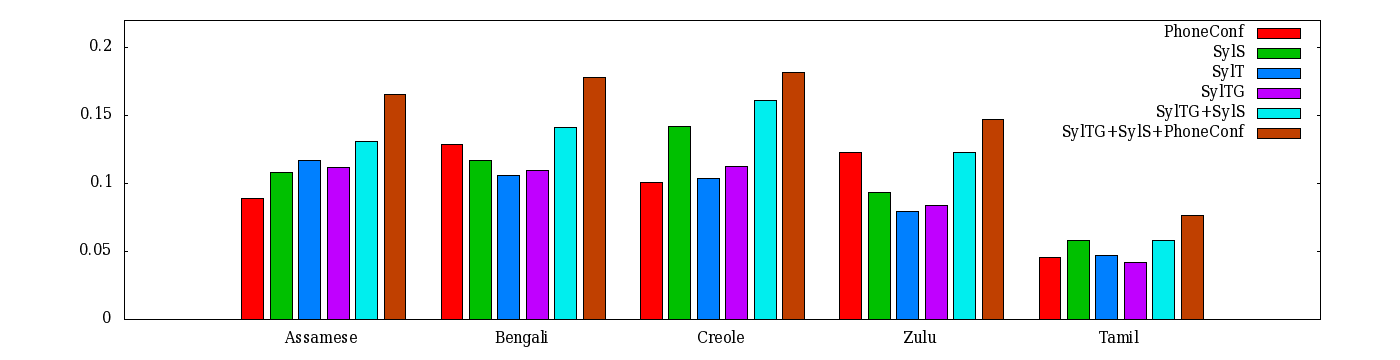
\includegraphics[width=1.00\textwidth, height=0.25\textwidth]{histall.png}
  \caption{OOV ATWV for different languages}
  \label{fig:atwvoov}
\end{figure*}

To get a feeling for the characteristics of these three methods, we present miss rate and false alarm rate on Assamese
in Table~\ref{tab:Miss}. It shows that the syllable transduction method tends to give lower false alarm rate, indicating
more accurate hypotheses.
\begin{table}[!t]
  \caption{PMiss and PFA for Assamese}
  \label{tab:Miss}
  \centering
  \begin{tabular}{cccc}
    \hline
              & PhoneConf & SylS  & SylT  \\
    \hline
    PMiss     & 0.853     & 0.827 & 0.859 \\
    PFA       & 0.00006   & 0.00006 & 0.00003 \\
    \hline
  \end{tabular}
\end{table}

\subsubsection{Combination}
Figure~\ref{fig:atwvoov} also shows the OOV ATWV on system combination. It is shown that system combination can effectively
improves the OOV ATWV.

\subsection{Analysis}
The phone confusion method usually generates many more hypotheses than the other two methods, giving a higher hit rate as well as
false alarm rate. The generated index file is usually much bigger than the other two methods, and it slows down the KWS. 
In addition, it uses the dev set for confusion matrix estimation, which makes tuning of hyper-parameters a bit complicated.

Syllable search usually generates a reasonable amount of hypotheses and gives good search results on OOV keywords. This
method does not require post-processing for syllable lattices. On the other hand, searching syllables in lattices 
usually takes more time than searching in word lattices, especially when lattices are dense.

Compared with the above methods, syllable transduction usually gives fewer but more accurate hypotheses, and is good 
at spotting both IV and OOV keywords. It has been shown that combination of a word system and a syllable transduction 
system gives better results than combining the word system with syllable search \cite{hang2014syllable}. This method 
also provides word lattices that are useful for OOV recognition. While it does not require any modification 
of the KWS template, this method requires a G2S system and a boosted language model for better performance. 

In general, these three methods combine well in terms of ATWV. This combination strategy does not require
training multiple acoustic models, which reduces the training time and computation greatly.

\section{Conclusion}
We show that syllable transduction is helpful in handling OOVs in low resources KWS tasks. 
Its good performance in both IV and OOV ATWV makes it a serious alternative to direct-searching in subword lattices. 
A keyword boosted language model further improves ATWV by mixing in unigram trained from keywords. Future 
work may benefit from improving syllable decoding accuracy, adding in more OOV pronunciations, and developing a
composition algorithm that preserves time information in lattices.

% use section* for acknowledgment
\section*{Acknowledgment}
The author would like to thank Ryan Yanzhang He and Eric Fosler-Lussier for their help on implementing 
the framework of G2P, and thank Brian Hutchinson, Peter Baumann and Aaron Jaech for their help on 
boosted language model. We also thank Korbinian Riedhammer for his generous help on syllable decoding, 
and Daniel Povey for his enlightening advice on lattice alignment.

% Can use something like this to put references on a page
% by themselves when using endfloat and the captionsoff option.
\ifCLASSOPTIONcaptionsoff
  \newpage
\fi

% trigger a \newpage just before the given reference
% number - used to balance the columns on the last page
% adjust value as needed - may need to be readjusted if
% the document is modified later
%\IEEEtriggeratref{8}
% The "triggered" command can be changed if desired:
%\IEEEtriggercmd{\enlargethispage{-5in}}

% references section

% can use a bibliography generated by BibTeX as a .bbl file
% BibTeX documentation can be easily obtained at:
% http://www.ctan.org/tex-archive/biblio/bibtex/contrib/doc/
% The IEEEtran BibTeX style support page is at:
% http://www.michaelshell.org/tex/ieeetran/bibtex/
% argument is your BibTeX string definitions and bibliography database(s)
%\bibliography{IEEEabrv,../bib/paper}

\bibliographystyle{IEEEtran}
\bibliography{journal}
%
% <OR> manually copy in the resultant .bbl file
% set second argument of \begin to the number of references
% (used to reserve space for the reference number labels box)

 
% If you have an EPS/PDF photo (graphicx package needed) extra braces are
% needed around the contents of the optional argument to biography to prevent
% the LaTeX parser from getting confused when it sees the complicated
% \includegraphics command within an optional argument. (You could create
% your own custom macro containing the \includegraphics command to make things
% simpler here.)
\begin{IEEEbiography}[{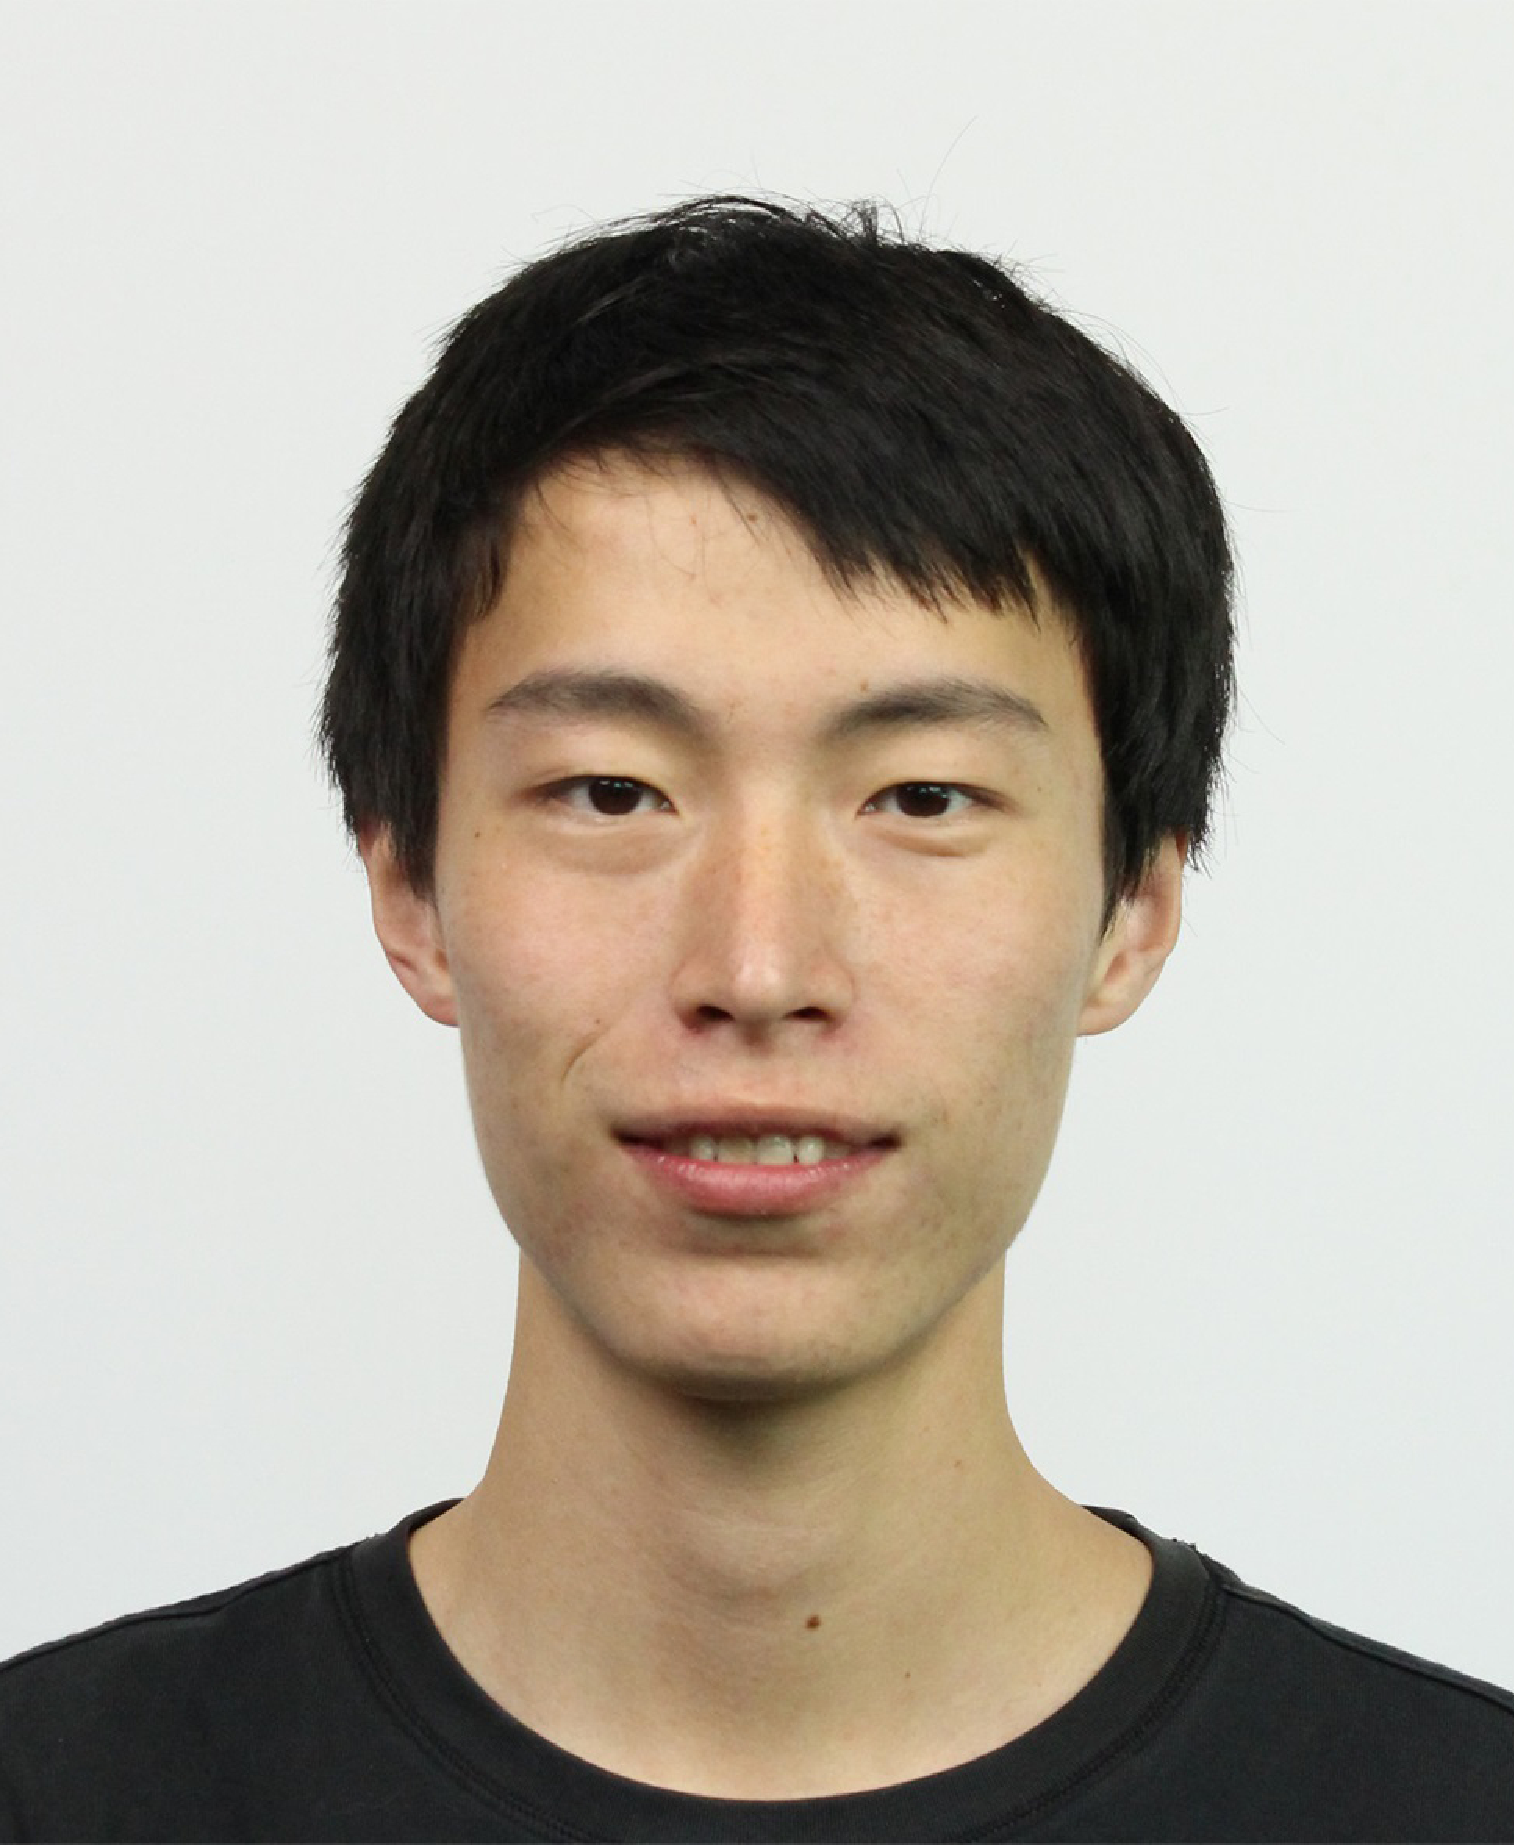
\includegraphics[width=1in,height=1.25in,clip,keepaspectratio]{hang}}]%
{Hang Su} received his B.E. degree from Tsinghua University, Beijing, China.
He is now a Ph.D. student in Department of Electrical Engineering \& Computer Science, 
University of California, Berkeley, CA, USA.
\end{IEEEbiography}

\begin{IEEEbiography}[{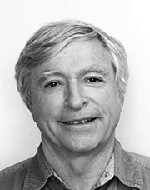
\includegraphics[width=1in,height=1.25in,clip,keepaspectratio]{james}}]%
{James Hieronymus} received his bachelor’s degree in physics from the University of Michigan at Ann Arbor, his master’s degree from UC San Diego, and his doctorate from Cornell University.
He held postdoctoral fellowships at Cornell and Stanford Artificial Intelligence Lab and supervisory positions at Heuristics Inc., an early speech recognition company. From 1982 to 1988, he was a computer scientist at the National Bureau of Standards (now the National Institute of Standards and Technology), where he helped establish the speech group.
\end{IEEEbiography}


% insert where needed to balance the two columns on the last page with
% biographies
%\newpage


% You can push biographies down or up by placing
% a \vfill before or after them. The appropriate
% use of \vfill depends on what kind of text is
% on the last page and whether or not the columns
% are being equalized.

%\vfill

% Can be used to pull up biographies so that the bottom of the last one
% is flush with the other column.
%\enlargethispage{-5in}



% that's all folks
\end{document}


